\documentclass[9pt]{beamer}
\usepackage{kotex}
\usepackage{amsfonts,amssymb,amsthm}
\usepackage[dvipsnames]{xcolor}
\usepackage{xcolor}
\usepackage{etoolbox}
\usepackage{braket}
\usepackage{qcircuit}

%## color
\definecolor{customBlack}{HTML}{3B4252}
\definecolor{customBlackGrey}{HTML}{434C5e}
\definecolor{cuatomGrey}{HTML}{4C566A} 
\definecolor{customWhite}{HTML}{ECEFF4} 
\definecolor{customBlue}{HTML}{6082B6}  
\definecolor{customRed}{HTML}{BF616A}
\definecolor{vividauburn}{rgb}{0.58, 0.15, 0.14}


%## Theme & custom
% \usetheme{metropolis}           % Use metropolis theme
% \metroset{block=fill}
\usetheme{moloch} % modern fork of the metropolis theme
\molochset{block=fill}
\setbeamersize{text margin left=5mm, text margin right=5mm}
\setbeamercolor{palette primary}{bg=customBlack}
\setbeamercolor{alerted text}{fg=customRed}
\setbeamercolor{itemize item}{fg=customBlue}
\setbeamercolor{enumerate item}{fg=customBlue}


%## font
\usefonttheme[onlymath]{serif}
% \setbeamerfont{normal text}{size=\small}
% \setbeamerfont{math text}{size=\tiny}


%## Theorem title, numbering
\makeatletter
\setbeamertemplate{theorem begin}
{%
\begin{\inserttheoremblockenv}
{%
\inserttheoremheadfont
\inserttheoremname
\ifx\inserttheoremaddition\@empty\else\ of\ \inserttheoremaddition\fi%
\inserttheorempunctuation
}%
}
\setbeamertemplate{theorem end}{\end{\inserttheoremblockenv}}
\makeatother
\setbeamertemplate{theorems}[numbered]  


%## Custom block
\setbeamercolor{block title}{bg=customBlue, fg=white}
\setbeamercolor{block body}{bg=customWhite, fg=customBlack}
\setbeamercolor{block title alerted}{%
    use={block title, alerted text},
    bg=customRed,
    fg=white
}
\setbeamercolor{block body alerted}{%
    use={block title, alerted text},
    bg=customWhite,
    fg=customBlack
}
\AtBeginEnvironment{definition}{%
    \setbeamercolor{block title}{fg=white,bg=customBlackGrey}
    \setbeamercolor{block body}{fg=customBlack, bg=customWhite}
}
\AtBeginEnvironment{theorem}{%
    \setbeamercolor{block title}{fg=white,bg=customBlackGrey}
    \setbeamercolor{block body}{fg=customBlack, bg=customWhite}
}
\AtBeginEnvironment{corollary}{%
    \setbeamercolor{block title}{fg=white,bg=customBlackGrey}
    \setbeamercolor{block body}{fg=customBlack, bg=customWhite}
}
\AtBeginEnvironment{lemma}{%
    \setbeamercolor{block title}{fg=white,bg=customBlackGrey}
    \setbeamercolor{block body}{fg=customBlack, bg=customWhite}
}


%! Useful command
\renewcommand{\Pr}{\text{Pr}}
% $\ast$ \underline{Proof}:
%\checkmark \underline{meaning}:

\title{4. Method of Types, Strong AEP and Universal Source Coding}
\date{\today}
\author{Vaughan Sohn}
% \institute{Centre for Modern Beamer Themes}


\begin{document}
    %#################################### 
    \maketitle
    
    %#################################### 
    \begin{frame}
        \frametitle{Contents}
        \tableofcontents
    \end{frame}


    \begin{frame}
        \frametitle{Lecture overview}
        \textbf{Overview}
        \vspace{0.4cm}
        \begin{itemize}
            \item 지금까지 우리는 source data의 true distribution을 알고 있다는 가정안에서 optimal인 source coding 방법에 대해서 소개했었다.
            \item 이번에는 실제 상황과 유사한, source의 true distribution을 모를 때의 source coding을 살펴보려고 한다. $\rightarrow$ \textit{Universal source coding theorem}
            \item Universal source coding theorem을 다루기 위하여 large deviation theory에서 사용되는 \alert{type}이라는 개념을 도입하고자한다.
            \item Type을 사용하면 weak typical set의 \textit{subset}인 strong typical set을 정의할 수 있고 strong typical set의 성질을 활용하여 universal source coding theorem을 증명하고자 한다.
        \end{itemize}
    \end{frame}


    %#################################### 
    \begin{section}{Types}
        \begin{frame}
            \frametitle{Limitation of weak typical set}
            \begin{itemize}
                \item Lecture 3에서 소개한 weak typical set은 다음과 같이 정의된다.
                $$ A^{(n)}_{\delta} (P) = \{x^n \in \mathcal X^n \ : \ e^{-n(H(P)+\delta)} \le P^n(x^n) \le e^{-n (H(P)-\delta)}\}$$
                \item $X_i \sim \operatorname{Bern}(1/2)$인 상황을 가정하자. ($p(0) = 1/2, p(1) = 1/2$)
                \item 그렇다면, 어떠한 sequence에 대해서도 다음이 성립하게 된다.
                $$e^{-n(H(P)+\delta)} \le P^n(x^n)  = {2^{-n}} \le e^{-n(H(P)-\delta)}$$
                $\Rightarrow$ sample space 전체가 weak typical set에 해당하게 된다! (something strange ...)
                \item 또한 weak typical set에 있는 sample이라고해서 반드시 Empirical distribution이 true distribution과 유사다하는 보장이 존재하지 않는다.
            \end{itemize}

            \vspace{0.2cm}
            \begin{block}{Idea of strong typical set}
                어떤 sample $x^n$에서 각 symbol이 나타난 횟수가 실제 true distribution과 유사한 sample들만을 모아서 strong typical set을 정의하고자한다.
                $$ N(a | x^n) \sim n P(a),\quad \forall a$$
            \end{block}
            
        \end{frame}

        \begin{frame}
            \frametitle{Empirical discrete probability distribution}
            \begin{definition}[empirical probability distribution]
                For $x^n \in X^n$, we denoted \textbf{empirical distribution} of $x^n$ as $\hat{P}_{x^n}$,
                $$\hat{P}_{x^n}(a) =\frac{1}{n} \sum_{i=1}^n \mathbf{1}\left(x_i=a\right) =\frac{1}{n} N\left(a | x^n\right) , \quad \forall a \in X  $$ where $N\left(a | x^n\right)$ is the number of $a$ 's in the given string $x^n$.
            \end{definition}
            \vspace{0.2cm}
            \checkmark \underline{meaning}: 실제로 우리가 얻을 수 있는 하나의 sample $x^n$에서 각 symbol이 등장한 \alert{횟수}($\ast$)를 세어 추정한 probability distribution.
            \\$\rightarrow$ 즉, empirical distribution은 $x^n$이라는 realized value에 의존한다. 
            \vspace{0.2cm}
            \begin{definition}[set of valid empirical probability distribution]
                Let $\mathcal{P}_n$ be the set of all valid empirical distributions over $X$ for a sequence of length $n$.
            \end{definition}
            \vspace{0.2cm}
            Example: $X = \{0, 1\}$
            $$ \mathcal P_n = \Big\{ \qquad \qquad \qquad \qquad \qquad \qquad \qquad \qquad \qquad\qquad \qquad \qquad \Big\}$$
        \end{frame}

        \begin{frame}
            \frametitle{Types}
            \begin{definition}[type]
                For a distribution $P \in \mathcal P_n$, the type $T_P$ is a set of length $n$ sequences that have empirical distribution $P$. 
                $$ T_P \triangleq \{ x^n \in \mathcal X^n \ : \  \hat P_{x^n} = P\},\quad T_P \subseteq \mathcal X^n$$
            \end{definition}
            \vspace{0.2cm}
            \checkmark \underline{meaning}: 특정 empirical distribution을 가지는 $x^n$들의 집합.
            \vspace{0.2cm}
            \begin{itemize}
                \item sequence에서 각 symbol들이 등장하는 횟수만 동일하다면, symbol의 순서가 달라도 동일한 type에 속하게 될 것이다. (e.g., $T_P = \{001, 010, 100\}$)
                \item Example: $X = \{0, 1\}, P = [\frac{k}{n}, \frac{n-k}{n}]$일 때, type의 크기는?
                \vspace{0.2cm}
                $$ |T_P| = \qquad \qquad.$$
            \end{itemize}

        \end{frame}


        \begin{frame}
            \frametitle{Types : size}
            \begin{theorem}[number of types]
                The number of types (=size of valid empirical probability distribution set) have loose upper bound:
                $$ \left|\mathcal{P}_n\right| \leq(n+1)^{|\mathcal X|} . $$
            \end{theorem}
            
            \begin{theorem}[size of each type]
                For any type $T_P$, ($P \in \mathcal P_n$)
                $$  \left|T_P\right|  \doteq e^{n H(P)}  $$
                where $|\mathcal X|=M$ and $\mathcal X=\left\{a_1, a_2, \ldots, a_M\right\}$.
            \end{theorem}

            \vspace{0.2cm}
            \checkmark \underline{meaning}: $n$이 커질수록, type의 크기가 증가하는 속도는 $H(P)$에 의해 조절된다.\\ \textit{rare한 event일수록 type의 크기가 증가하는 속도도 느리다!}
            \begin{itemize}
                \item if $H(P) \downarrow$ then $e^{nH(P)} \downarrow$
                \item if $H(P) \uparrow$ then $e^{nH(P)} \uparrow$
            \end{itemize}
        \end{frame}

        \begin{frame}
            \frametitle{Types : size}
            To prove Theorem 5, we will use \textit{Stirling's approximation}.
            \begin{lemma}[Stirling’s approximation]
                $$ n!\approx \sqrt{2 \pi n} \cdot n^n e^{-n} $$ 
                More precisely, 
                $$ \lim _{n \rightarrow \infty} \frac{n!}{\sqrt{2 \pi n} \cdot n^n e^{-n}}=1 $$
                Or even more precisely,
                $$ \sqrt{2 \pi n} \cdot n^n e^{-n} e^{\frac{1}{12 n+1}} \leq n!\leq \sqrt{2 \pi n} \cdot n^n e^{-n} e^{\frac{1}{12 n}} $$
            \end{lemma}
        \end{frame}
        
        \begin{frame}
            \frametitle{Types : size}
            
            $\ast$ \underline{Proof} (Theorem 5): 
            $$
            \begin{aligned}
            \left|T_P\right| & =\binom{n}{n P\left(a_1\right), n P\left(a_2\right), \ldots, n P\left(a_M\right)} \\
            & =\frac{n!}{\prod_{i=1}^M\left(n P\left(a_i\right)\right)!} \\
            & \doteq \frac{n^n e^{-n} \sqrt{2 \pi n}}{\prod_{i=1}^M\left(n P\left(a_i\right)\right)^{n P\left(a_i\right)} e^{-n P\left(a_i\right)} \sqrt{2 \pi n P\left(a_i\right)}} \\
            & \doteq \frac{1}{\prod_{i=1}^M P\left(a_i\right)^{n P\left(a_i\right)}}=\frac{1}{\prod_{i=1}^M e^{n P\left(a_i\right) \log P\left(a_i\right)}}=e^{n H(P)} .
            \end{aligned}
            $$
        \end{frame}

        \begin{frame}
            \frametitle{Types : probability}
            \begin{theorem}[probability of any sequence in the type]
                If the probability of the sequence under the \textbf{true} distribution $Q^n$ ($X_i \sim Q$), 
                then $Q^n\left(x^n\right)$ is all the same for all $x^n \in T_P$.
                and the probability is:
                $$Q^n\left(x^n\right)=e^{-n[H(P)+D(P \| Q)]} $$ 
            \end{theorem}
            \vspace{0.2cm}
            \checkmark \underline{meaning}:
            만약 실제 $X_i$가 i.i.d $Q$ distribution을 따른다면, 동일한 type set $T_P$안에 들어있는 sequence들의 probability $Q^n(x^n)$은 전부 동일하다.
            \vspace{0.2cm}
            \\$\ast$ \underline{Proof}:
            $$ 
            \begin{aligned}
                Q^n\left(x^n\right) & =\prod_{i=1}^n Q\left(x_i\right) =\prod_{a \in \mathcal X} Q(a)^{N\left(a \mid x^n\right)} =\prod_{a \in \mathcal  X} Q(a)^{n P(a)} \\
                & = \exp\left(\log \bigg[\prod_{a \in \mathcal  X} Q(a)^{n P(a)} \bigg]\right) = \exp \left( n \sum_{a \in \mathcal  X} P(a) \log Q(a) \right) \\
                & = \exp \Big( n \sum_{a \in \mathcal  X} P(a) \log P(a)  - (P(a) \log P(a) - P(a) \log Q(a)) \Big) \\&= \boxed{e^{-n[H(P) + D(P\| Q)]}}
            \end{aligned}
            $$ 
        \end{frame}
        

        \begin{frame}
            \frametitle{Types : probability}
            \begin{corollary}[probability of the type]
                $$Q^n(T_P) \doteq e^{-nD(P||Q)}$$
            \end{corollary}
            \vspace{0.2cm}
            $\ast$ \underline{Proof}: (hint. using Theorem 5, 7)
            \\$\Rightarrow$
            \vspace{1cm}
            \begin{lemma}[probability of any sequence in the empirical type and true type]
                Probability of any sequence $x_n, (X_i \sim Q)$ in the type with empirical distribution $P$ and true distribution $Q$ is satisfies the following inequality:
                $$Q^n(T_Q) \ge Q^n (T_P),\qquad \forall P, Q \in \mathcal P_n$$ 
            \end{lemma}
            $\ast$ \underline{Proof}: (hint. using $\frac{n!}{m!} \leq n^{n-m} $)
            \\$\Rightarrow$
            \vspace{1cm}
        \end{frame}

        \begin{frame}
            \frametitle{Some remarks}
            \begin{itemize}
                \item 각 type은 그 정의에 의하여 sample space $\mathcal X^n$에 대하여 서로 disjoint하며 collectively exhaustive하므로 $\mathcal X^n$의 \textit{partitions}이다.
                ($ \bigcup_{P \in \mathcal P_n} T_P $)
                \item $\mathcal P_n$의 크기에 대한 bound는 loose한 bound이지만, 이 theorem으로부터 types의 개수가 sequence의 길이 $n$에 대해 \textbf{polynomial}하게 증가한다는 것을 알 수 있다. 
                \item 그러나 $\mathcal X^n$을 이루는 각각의 disjoint set $T_P$는 크기가 $n$에 대해 exponential하게 증가하며, 증가속도는 $H(P)$에 의해 결정된다.
                \item 또한, 동일한 type에 속하는 sequence들의 확률은 모두 동일하며, 그 값은 $n$에 대해 exponential하게 감소한다. 감소속도는 empirical distribution $P$가 true distribution $Q$와 얼마나 가까운지에 따라 결정된다.
                \item 만약 두 확률이 거의 유사하다면 $(D(P||Q) \downarrow)$, type $T_P$에 있는 sample들이 발생할 확률은 $n$에 따라 빠르게 증가하게 된다.
                \item $P=Q$일 때, Corollary 8에 의하면 $Q^n (T_Q) \doteq 1$을 얻을 수 있지만, 이는 $T_Q$의 확률이 exponential하게 증가하거나 감소하지 않는다는 사실만을 의미할 뿐, 아무런 정보도 우리에게 주지 않는다. 
                $$ Q^n(T_Q) \doteq 0 \doteq 1 \doteq e^0 \cdots$$
            \end{itemize}
            \vspace{-0.5cm}
        \end{frame}

        \begin{frame}
            \frametitle{Summary}
            \begin{block}{Summary of Types}
                Type; a new way of classifying length $n$ sequences.
                \begin{itemize}
                    \item $T_P \triangleq\big\{x^n \in \mathcal{X}^n: \hat{P}_{x^n}=P\big\}$
                    \item $\left|T_P\right| \doteq e^{n H(P)}$
                    \item $Q^n\left(x^n\right)=e^{-n(H(P)+D(P \| Q))} \quad \text { for } x^n \in T_P $
                    \item $Q^n\left(T_P\right) \doteq Q^n\big(\big\{x^n: \hat{P}_{x^n}=P\big\}\big)=e^{-n D(P \| Q)}$
                \end{itemize}
                
            \end{block}
        \end{frame}
    \end{section}




    %#################################### 
    \begin{section}{Method of Types}
        \begin{frame}
            \frametitle{Method of types : size}
            이제 하나의 type이 아니라 여러가지 type들의 union set에 대하여 분석해보자.

            \begin{itemize}
                \item Type은 서로 disjoint하기 때문에 다음을 만족한다. (\textit{assume} $H(P_1) > H(P_2)$)
                $$ e^{n H(P_1)} \le |T_{P_1} \cup T_{P_2}| = |T_{P_1}| + |T_{P_2}| \doteq e^{nH(P_1)} + e^{nH(P_2)}  \le {2}e^{nH(P_1)} \doteq \boxed{ e^{nH(P_1)}}$$ %2가 const니까
                \item $M$개의 type으로 일반화 하면, 다음과 같다. (\textit{assume} $H(P_1) \ge H(P_i), \forall i$)
                $$
                e^{n H\left(P_1\right)} \leq\left|\bigcup_{i=1}^M T_{P_i}\right| \leq M\left|T_{P_1}\right| \doteq {M e^{n H\left(P_1\right)}} \doteq \boxed{ e^{n H\left(P_1\right)}}
                $$
                $\Rightarrow$ Theorem 5에 의하면, type의 개수는 \alert{polynomial}이기 때문에, 위와 같은 approximation이 가능하다. ($M \not \doteq e^n$)
                \item 더 나아가, 이를 이용하면 어떤 특별한 constraint를 만족하는 type들의 union set $\mathcal A$에 대한 크기도 표현할 수 있다. (assume $P^*=\underset{P \in \mathcal A}{\arg \max } H(P)$)
                
                $$
                \left|\bigcup_{P \in \mathcal{A}} T_P\right|=\sum_{P \in \mathcal{A}}\left|T_P\right| \doteq \sum_{P \in \mathcal{A}} e^{n H(P)} \doteq \boxed{ e^{n H\left(P^*\right)}}
                $$

            \end{itemize}
        \end{frame}

        \begin{frame}
            \frametitle{Method of types : probability}
            \begin{theorem}[Sanov's theorem]
                Let $Q$ be a distribution over $\mathcal X$. Let $\mathcal A$ be a set of distributions over $\mathcal X$, and suppose that $Q \notin \mathcal A$:
                $$ Q^n\left(\left\{x^n: \hat{P}_{x^n} \in \mathcal{A}\right\}\right) \doteq e^{-n \min _{P \in \mathcal{A}} D(P \| Q)} $$
            \end{theorem}
            \vspace{0.2cm}
            $\ast$ \underline{Proof}: hint. union type set의 크기를 구하기 위해 적용했던 과정을 그대로 확률에도 적용하면, 쉽게 증명할 수 있다.
            $$
            e^{-n D(P^{**} \| Q)} \doteq Q^n\left(T_{P^{**}}\right) \leq Q^n\left(\bigcup_{P \in \mathcal{A}} T_P\right) \leq(n+1)^{|\mathcal X|} Q^n\left(T_{P^{**}}\right) \doteq e^{-n D(P^{**} \| Q)}
            $$
            \textit{where}
            $$
            P^{* *}=\underset{P \in \mathcal{A}}{\arg \min } D(P \| Q)
            $$

        \end{frame}

        \begin{frame}
            \frametitle{Some remarks \& Summary}
            \textit{Some remarks}
            \vspace{0.2cm}
            \begin{itemize}
                \item 특정한 조건을 만족하는 empirical probability들의 집합 $\mathcal A$를 다음과 같이 가정해보자.
                $$ \mathcal A \triangleq \{P \ : \ \mathbb E_P [F(X)] > \alpha \}$$
                $\Rightarrow$ $X$의 함숫값 $F(X)$들의 expectation이 threshold $\alpha$보다 크도록 하는 분포
                \item 집합 $\mathcal A$를 잘 정의하면, decode $F$를 했을 때 정확도가 $\alpha$보다 크도록 만드는, 또는 특정 error rate보다 더 작은 에러를 만들어내는 분포들의 집합을 정의할 수도 있다.
                \item 따라서 이런 아이디어를 바탕으로 strong typical set을 정의하고자한다.
            \end{itemize}
            \vspace{0.3cm}
            \begin{block}{Summary of method of types}
                \begin{itemize}
                    \item $|\bigcup T_P| \doteq e^{nH(P^*)}$ where $P^* = \arg\max H(P)$
                    \item $Q^n(\bigcup T_P) \doteq e^{-nD(P^{**} \| Q)}$ where $P^{**} = \arg\min D(P\| Q)$
                \end{itemize}
            \end{block}
        \end{frame}
    \end{section}




    %#################################### 
    \begin{section}{Strong Typicality}
        \begin{frame}
            \frametitle{Strong typical set}
            \begin{definition}[strong typical set]
                For a given distribution $Q$ with $Q(x)>0, \forall x$, and a constant $\delta>0$, the \textbf{strong typical set} is defined as 
                $$ \tilde{T}_Q= \bigcup_{P \in \mathcal A} T_P=\bigcup_{\{P : |P(x)-Q(x)| \leq \delta, \forall x \}} T_P $$
                where $\mathcal A$ is defined 
                $$ A = \{P : |P(x) - Q(x)| \le \delta, \forall x \in \mathcal X\}$$
            \end{definition}
            \vspace{0.2cm}
            \checkmark \underline{meaning}: source에 속하는 모든 symbol $x$에 대하여, true distribution과의 차이가 $\delta$보다 작은 empirical distribution들의 집합 $\mathcal A$에 대한 union type set.
            \begin{itemize}
                \item $P(x) = \frac{1}{n} \sum^n_{i=1} \mathbf 1 (x_i = x)$
                \item $Q(x) = \mathbb E_{Q}[\mathbf 1 (x_i = x)]$
            \end{itemize}


        \end{frame}

        \begin{frame}
            \frametitle{Strong AEP}
            \begin{theorem}[Strong AEP]
                For any $\epsilon$, $\delta>0$, there exists a $N_0$ s.t. $\forall n > N_0$,
                $$
                Q^n(\tilde{T}_Q)>1-\epsilon
                $$
                more precisely,
                $$ Q^n (\tilde T_Q) \rightarrow 1. $$
            \end{theorem}
            \vspace{0.2cm}
            \checkmark \underline{meaning}: 특정 sample이 strong typical set에 속할 확률은 1로 수렴한다.
            \vspace{0.2cm}
            \\$\ast$ \underline{Proof}: (hint. using WLLN, union bound)
            \begin{itemize}
                \item $Q^n(\tilde T_Q) \rightarrow 1$임을 보이는 대신, $Q^N(\tilde T_Q^C) \rightarrow 0$임을 보이고자한다.
                $$ Q^n\left(\left\{x^n:\left|\hat{P}_{x^n}(a)-Q(a)\right|>\delta \text { for some } a \in \mathcal{X}\right\}\right) \rightarrow 0 . $$
                \item 어떤 \textit{특정한} $a \in \mathcal X$에 대하여 WLLN을 적용하면 다음을 보일 수 있다.
                $$ Q^n\left(\left\{x^n:\left|\hat{P}_{x^n}(a)-Q(a)\right|>\delta\right\}\right)<\frac{\epsilon}{|\mathcal{X}|}$$ 
            \end{itemize}
        \end{frame}

        \begin{frame}
            \frametitle{Strong AEP}
            $\ast$ \underline{Proof}: (contd.)
            \begin{itemize}
                \item Union bound를 적용하면, for some $a$에 대한 확률은 for any $a\in \mathcal X$에 대한 확률들의 합으로 bound된다.
                $$ \begin{aligned}
                    & Q^n\left(\left\{x^n:\left|\hat{P}_{x^n}(a)-Q(a)\right|>\delta \text { for some } a \in \mathcal{X}\right\}\right) \\
                    & \leq \sum_{a \in \mathcal{X}} Q^n\left(\left\{x^n:\left|\hat{P}_{x^n}(a)-Q(a)\right|>\delta\right\}\right) \\
                    & \leq \epsilon.
                \end{aligned} $$
                \item 따라서 $Q^n(\tilde T_Q)$의 complement가 $\epsilon$으로 bound되므로 다음을 얻는다.$\Box$
                $$ Q^n(\tilde T_Q) > 1-\epsilon.$$
            \end{itemize}
        \end{frame}

        % \begin{frame}
        %     \frametitle{Strong typical set size}
        %     Method of Types로 쉽게 증명이 가능함. 따라서 생략
        % \end{frame}

        \begin{frame}
            \frametitle{Comparison between weak typical set}
            \begin{columns}
                \begin{column}{0.5\textwidth}
                    \textbf{ weak typical set} $A^{(n)}_{\delta} (Q)$
                    \vspace{0.2cm}
                    {\footnotesize {$$  { \Big\{ x_1^n \in \mathcal X^n : \Big| - \frac{1}{n} \log Q^n (x^n_1) - H(Q) \Big| \le \delta \Big\}}$$}}
                    \begin{itemize}
                        \item $\forall x_1^n \in A_{\delta_n}^{(n)}(Q),\ Q^n (x^n) \doteq e^{-nH(Q)}$. % probability of typical set entry
                        \item $|A_{\delta_n}^{(n)} (Q)| \doteq e^{nH(Q)}$. % size of typical set
                        \item (weak AEP) $Q^n(A_{\delta_n}^{(n)}) \rightarrow 1$ \textit{with sufficiently large} $n$. % convergence probability of typical set
                    \end{itemize}
                \end{column}

                \begin{column}{0.5\textwidth}
                    \textbf{ strong typical set} $\tilde T_Q$
                    \vspace{0.2cm}
                    {\footnotesize {$$ { \Big\{ x_1^n \in \mathcal X^n : \big|\hat P_{x^n}(a) - Q(a)\big| \le \delta, \forall a \in \mathcal X \Big\}}$$}}
                    \begin{itemize}
                        \item $\forall x_1^n \in \tilde T_Q,\ Q^n (x^n) \doteq e^{-nH(Q)}.$
                        \item $|\tilde T_Q| \doteq e^{nH(Q)}.$
                        \item (strong AEP) $Q^n (\tilde T_Q) \rightarrow 1$ \textit{with sufficiently large} $n$.
                        \item \alert{$|\hat P_{x^n} (a) - Q(a) | < \delta, \forall a \in \mathcal X$}.
                    \end{itemize}
                \end{column} 
            \end{columns}
        \end{frame}

        \begin{frame}
            \frametitle{Summary}
                \begin{block}{Summary of strong typical set}
                    \begin{itemize}
                        \item empirical distribution과 true distribution의 값이 모든 symbol에 대해서 $\delta$보다 멀리 떨어지지 않도록 하는 constraint를 만족하는 probability에 대한 union type set으로 strong typical set을 정의할 수 있다.
                        \item method of types를 이용하면, strong typical set의 크기와 strong typical set에 속하는 모든 원소들의 확률이 weak typical set의 특징을 만족함을 보일 수 있다.
                        \item 즉, strong typical set에 속하는 data만 encoding하는 방식을 차용하면, strong typical set을 이용하여 source coding theorem을 증명할 수 있다.
                    \end{itemize}
                \end{block}
        \end{frame}
    \end{section}




    %#################################### 
    \begin{section}{Universal Source Coding}
        \begin{frame}
            \frametitle{Unknown distribution source}
            다음과 같이 \alert{unknown} distribution $Q$를 따르는 source data ($DMS(Q)$)에 대한 optimal block source coding 방법을 찾는 것이 목적이다.
            $$ \begin{aligned} &f_n: \mathcal{X}^n \rightarrow\{0,1\}^{n R}, \\ &g_n:\{0,1\}^{n R} \rightarrow \mathcal{X}^n \end{aligned}$$

            \begin{definition}[probability of error]
                The \textbf{probability of error} for the code with respect to the distribution $Q$ is
                $$ P_e^{(n)} \triangleq Q^n\left(\left\{x^n: g_n\left(f_n\left(x^n\right)\right) \neq x^n\right\}\right) .$$
            \end{definition}
            
            
        \end{frame}

        \begin{frame}
            \frametitle{Unknown distribution source}
            
            \begin{definition}[error exponent]
                We say that an \textbf{error exponent} $E$ is achievable at rate $R$ if there exists a sequence of $(n, R)$ codes with 
                $$P_e^{(n)}\  \dot {\le}\  e^{-nE},$$
                which means 
                $$\limsup_{ n \rightarrow \infty} \frac{1}{n} \log P_e^{(n)} \le -E.$$
            \end{definition}

            \begin{itemize}
                \item Unknown distribution이기 때문에 $H(P) > R$이더라도 $R$이 길어질수록 error probability 점차 0에 수렴할 뿐, 여전히 존재한다.
                \item 따라서 $R$이 커질 수록 error가 얼마나 빠르게 감소하는지를 표현하기 위해서 error exponent를 도입한다. (If $E \uparrow$, then error decreasing fast.)
            \end{itemize}

            \begin{figure}
                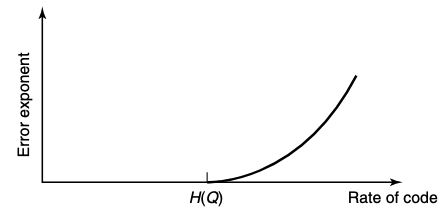
\includegraphics[width=0.55\textwidth]{image/L4_error_exponent.png}
            \end{figure}
        \end{frame}
        
        \begin{frame}
            \frametitle{Universal source codes}
            \begin{definition}[universal source codes]
                A rate $R$ block code for a source will be called \textbf{universal} if the functions $f_n$ and $g_n$ do not depend on the distribution $Q$ and if $P_\epsilon^{(n)} \rightarrow 0$ as $n \rightarrow \infty$ if \alert{$R>H(Q)$}.

            \end{definition}
            \begin{block}{Idea for universal source codes}
                \begin{itemize}
                    \item source coding theorem에 의하면, $H(Q) \le R$으로 설정하면 error가 0으로 수렴하도록 만들 수 있다.
                    \item 우리는 true distribution을 모르기 때문에, 대신 다음을 만족하는 \textit{empirical} probability set을 가정하자. % (단, 우리가 정한 R이 정말 H(Q)보다 큰 값인지는 알 수 없다.... Q를 모르기 때문임)
                    $$ \mathcal A = \{ P : H(P) \le R \}$$
                    \item $\mathcal A$에 대한 union type sets에 속하는 sample data들만 encoding하자!
                    $$ T_{\mathcal A} \triangleq \bigcup_{P \in \mathcal A} T_P = \{ x^n : H(\hat P_{x^n}) \le R \}$$
                \end{itemize}
            \end{block}
            
        \end{frame}

        \begin{frame}
            \frametitle{Universal source coding theorem}
            \begin{theorem}[universal source coding theorem]
                There exists a sequence of $(n, R)$ universal source codes such that $P_c^{(n)} \rightarrow 0$ for every source $Q$ such that $H(Q)<R$.  With this universal source coding, the achievable error exponent is
                $$
                E=\min _{P:  H(P)>R} D(P||Q),
                $$
                i.e.,  
                $$
                P_e^{(n)}\  \dot \leq \ e^{-n \min _{P:H(P)>R} D(P||Q)}. 
                $$
                
            \end{theorem}
            \vspace{0.2cm}
            $\ast$ \underline{Proof}: (hint. Sanov's theorem)
            \begin{itemize}
                \item 아이디어에서 소개했던 union type set $T_{\mathcal A}$에 대해 methods of types를 적용하면, 집합의 크기를 구할 수 있다.
                $$ \begin{aligned}
                    |T_{\mathcal A} | & =\sum_{P \in \mathcal{A}_n: H(P) \leq R}\left|T_P\right| \doteq \sum_{P \in \mathcal{A}_n: H(P) \leq R} e^{n H(P)} \\
                    & \leq(n+1)^{|X|} e^{n R}
                    \end{aligned} $$
            \end{itemize}
        \end{frame}

        \begin{frame}
            \frametitle{Universal source coding theorem}
            $\ast$ \underline{Proof}: (contd.)
            \begin{itemize}
                \item 우리가 고안한 방법은 $T_{\mathcal A}$에 속하는 sample에 대해서만 encoding을 수행하기 때문에, error probability는 다음과 같이 정의된다.
                $$ P_e^{(n)} =1-Q^n(A)  $$
                \item Method of types를 이용하면 $Q^n (T_P)$를 다음과 같이 전개할 수 있다.$\Box$
                $$ \begin{aligned}
                    P_e^{(n)} & =1-Q^n(A) \\
                    & =\sum_{P: {\color{red}H(P)>R}} Q^n\left(T_P\right) \\
                    & \leq(n+1)^{|X|} \max _{P: H(P)>R} Q^n\left(T_P\right) \\
                    & \leq(n+1)^{|X|} e^{-n \min _{P:  H(P)>R} D(P \| Q)} .
                    \end{aligned} $$
                \textit{where for $P$ that } $H(P) > R> H(Q)$?
            \end{itemize}
        \end{frame}


    \end{section}

    \begin{frame}{References}
        \begin{itemize}
            \item T. M. Cover and J. A. Thomas. Elements of Information Theory, Wiley, 2nd ed., 2006.
            \item Gallager (2008), Principles of Digital Communication, Cambridge University Press.
            \item Lecture notes for EE623: Information Theory (Fall 2024)
        \end{itemize}
        \vspace{6cm}
    \end{frame}


\end{document}